\documentclass[14pt]{article}

\usepackage[polish]{babel}
\usepackage[utf8]{inputenc}
\usepackage[T1]{fontenc}
\usepackage{extsizes}
\usepackage{graphicx}
\usepackage{tocloft}
\usepackage{amsmath}
\usepackage{multirow}
\usepackage{hyperref}


\font\titlefont=cmtt10 at 22pt

\title{
    
\includegraphics[scale=0.5]{images/logo-pwr-pion.png}
    \vspace{1cm}
    \\
    {\textbf{
    \titlefont Sygnały i obrazy cyfrowe
    \\ Laboratorium 2 - Skalowanie i rotacja
    }}
}
    
\author{
    Informatyczne Systemy Automatyki
    \\
    \\ Wykonujący:
    \\ Igor Potyrała - 272518
    \\
    \\ Prowadzący - Przemysław Śliwiński
}
\date{Data laboratoriów: 25 pażdziernika oraz 8 listopada 2023}


\begin{document}
\maketitle
\newpage
% Spis treści
%\newpage
%\renewcommand{\cftsecleader}{\cftdotfill{\cftdotsep}}
%{
 % \hypersetup{linkcolor=black, hidelinks}
 % \tableofcontents
%}

% Wstęp teoretyczny, definicje
\section{Zadania}
\subsection{Algorytmy interpolacji}
Celem zadania pierwszego było sprawdzenie działania 3 algorytmów interpolacji
do skalowania oraz obracania względem puntku. Każdy z algorytmów 
różni się metodą interpolacji wartości pikseli i złożnością obliczeniową.
Algorytmy te to:
\begin{itemize}
    \item Najbliższy sąsiad,
    \item Liniowa,
    \item Sześcienna
\end{itemize}



\newpage
\subsection{Skalowanie i rotacja}
\subsubsection{Wyniki skalowania}
\begin{center}
    \vspace{1.2cm}
    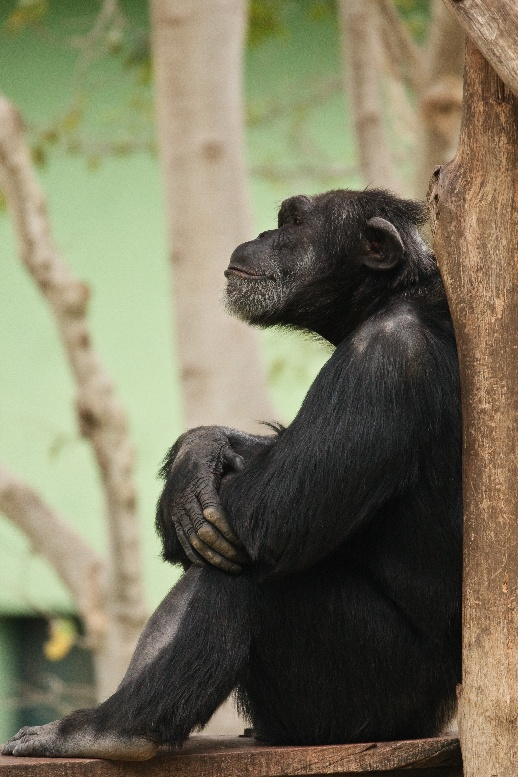
\includegraphics[scale=0.2]{images/monke_512.jpg}
    \\ \small Obraz 1. Oryginalny obraz.

    \vspace{1.5cm}
    \begin{minipage}{7cm}
        \begin{center}
            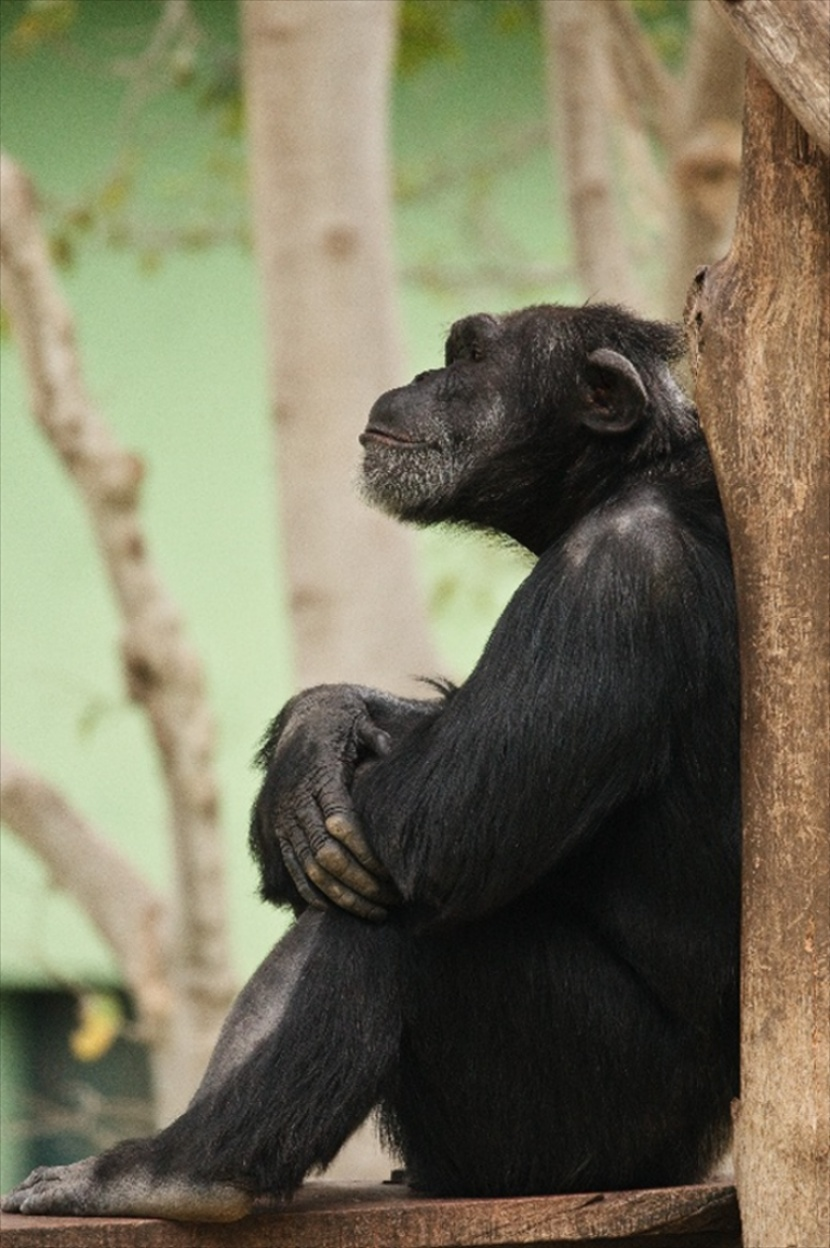
\includegraphics[scale=0.15]{images/5x_10_bc.jpg}
            \\ \small Obraz 2. 5-krotne powiększenie 
            \\o 10\% za pomocą interpolacji sześciennej.
        \end{center}
    \end{minipage}
    \hfill
    \begin{minipage}{7cm}
        \begin{center}
            \vspace{1.2cm}
            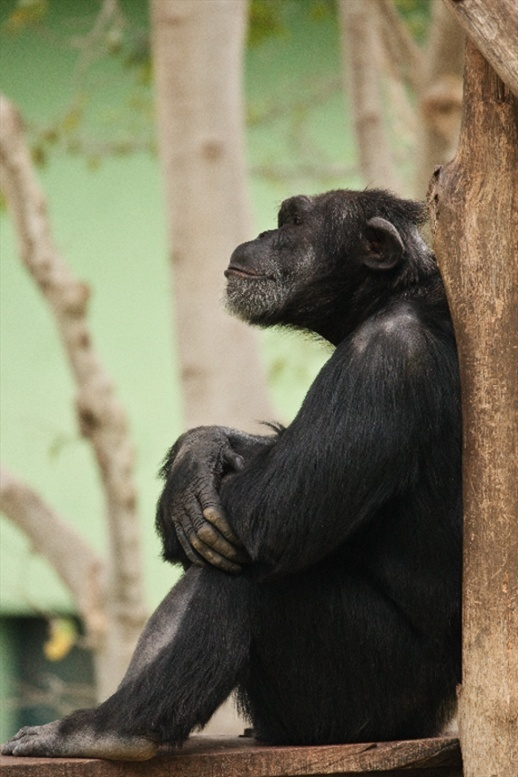
\includegraphics[scale=0.2]{images/5x_BACK_TO_ORG_bc.jpg}
            \\ \small Obraz 3. Pomniejszenie z powrotem do oryginalnej wielkości za pomocą 
            interpolacji sześciennej. 
      \end{center}
    \end{minipage}


    %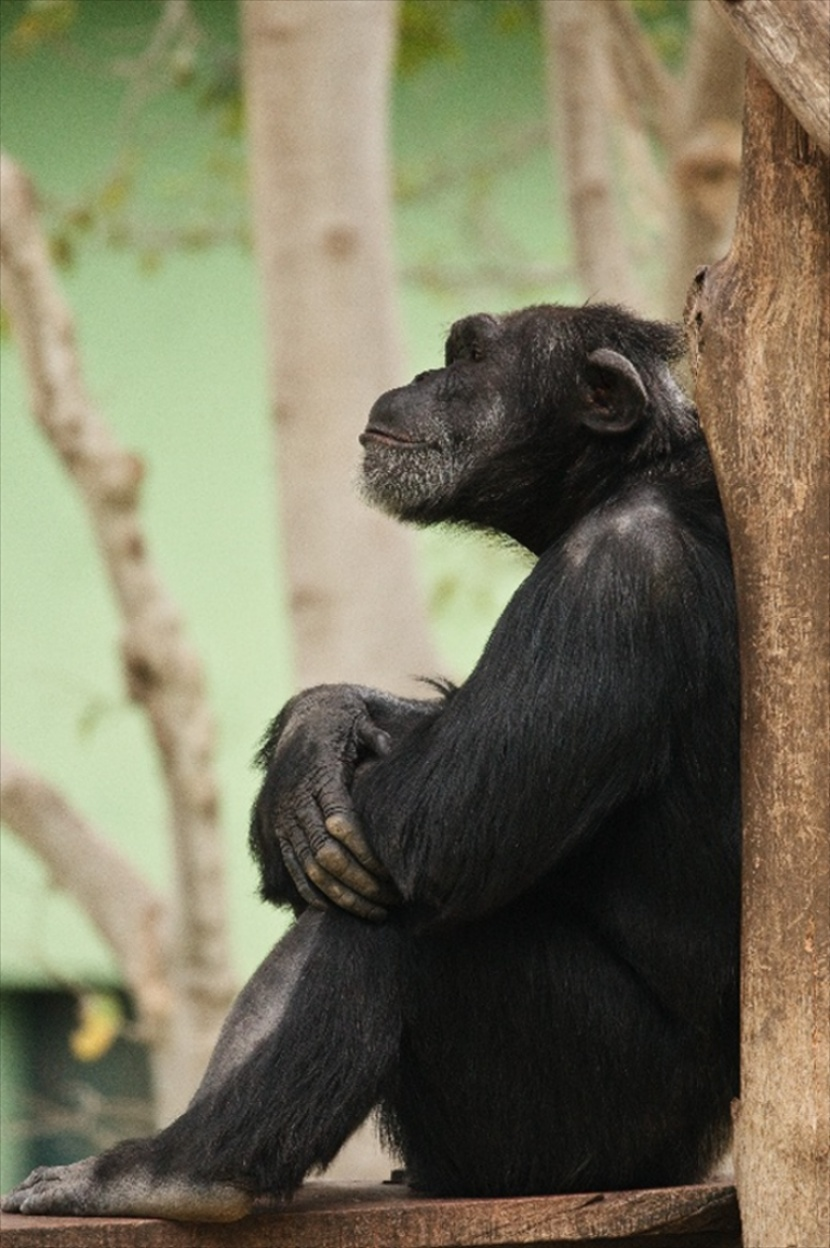
\includegraphics[scale=0.3]{images/5x_10_bc.jpg}
    %\\ \small Obraz 1. 5-krotne powiększenie o 10\% za pomocą 
    %interpolacji sześciennej.

    %\vspace{0.2cm}
    %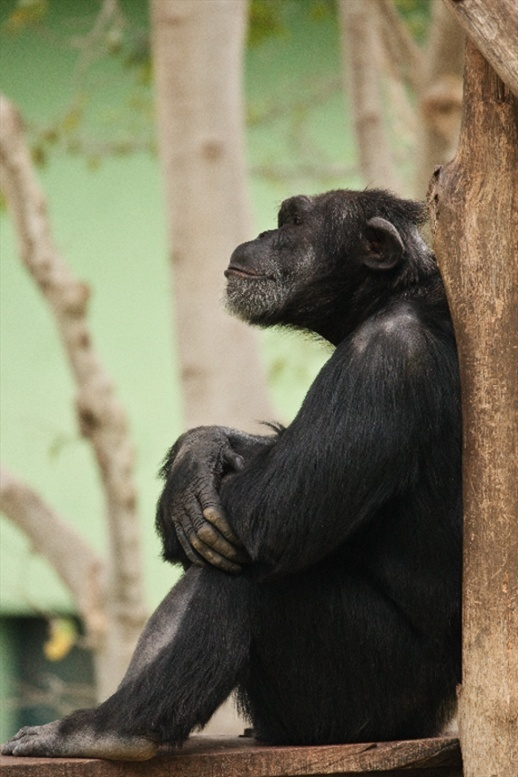
\includegraphics[scale=0.3]{images/5x_BACK_TO_ORG_bc.jpg}
    %\\ \small Obraz 2. Pomniejszenie z powrotem do oryginalnej wielkości za pomocą 
    %interpolacji sześciennej. 

    %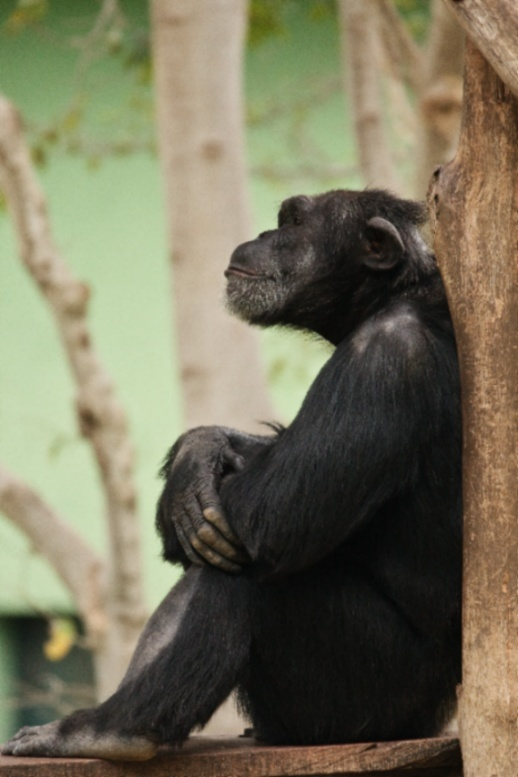
\includegraphics[scale=0.3]{images/5x_BACK_TO_ORG_bl.jpg}
    %\\ \small Obraz 3. 5-krotne powiększenie o 10\%, a następnie pomniejszenie
    %do oryginalnej wielkości -liniowa.

    %\vspace{0.2cm}
    %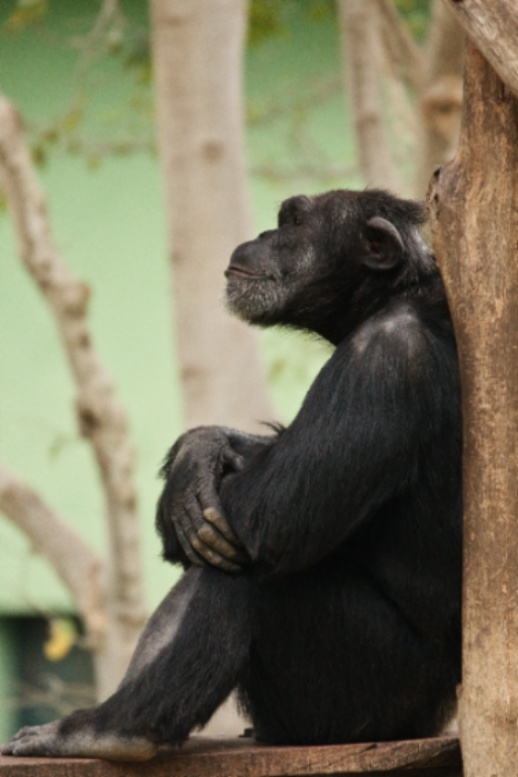
\includegraphics[scale=0.3]{images/3x_BACK_TO_ORG_bl.jpg}
    %\\ \small Obraz 4. 3-krotne pomniejszenie o 10\%, a następnie powiększenie
    %do oryginalnej wielkości - liniowa.

    %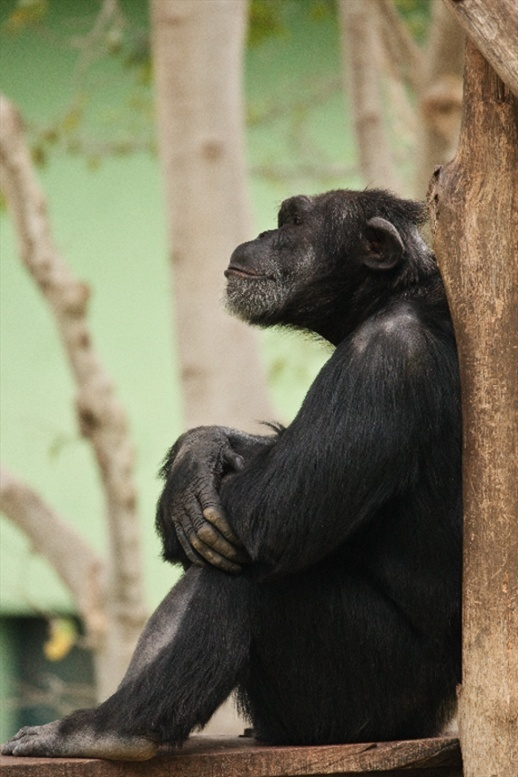
\includegraphics[scale=0.3]{images/5x_BACK_TO_ORG_bc.jpg}
    %\\ \small Obraz 5. 5-krotne powiększenie o 10\%, a następnie pomniejszenie
    %do oryginalnej wielkości - sześcienna.

    %\vspace{0.2cm}
    %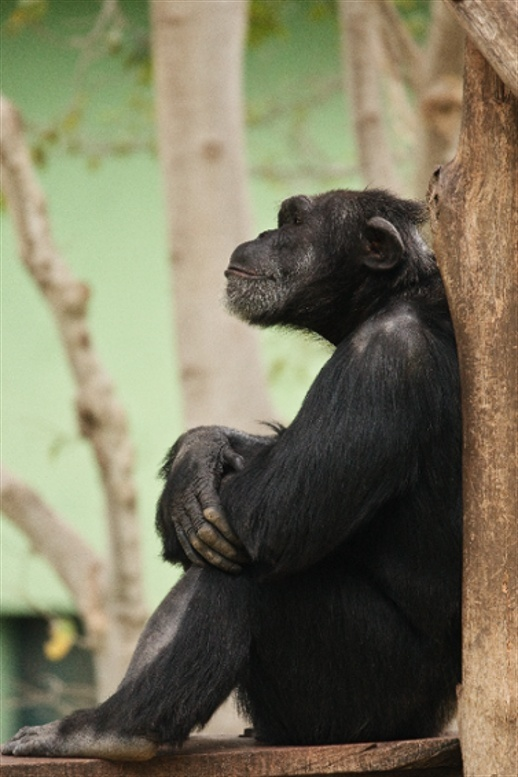
\includegraphics[scale=0.3]{images/3x_BACK_TO_ORG_bc.jpg}
    %\\ \small Obraz 6. 3-krotne pomniejszenie o 10\%, a następnie powiększenie
    %do oryginalnej wielkości - sześcienna.

    %\vspace{0.25cm}
    %\begin{tabular}{|c|c|c|c|}
        %\hline
        %& Najbliższy sąsiad & Liniowa & Sześcienna  \\ \hline
        %Powiększenie & 0,38s & 4,86s & 55,35s \\ \hline
        %Pomniejszenie & 0,27s & 2,77s & 40,51s \\ \hline
        %Średni błąd kwadratowy & 55,41 & 33,10 & 23,37 \\ \hline

    %\end{tabular}
    %\vspace{0.2cm}
    %\\ \small Tabela 1. Przedstawiające charakterystyki 
    %czasowe oraz błędy typów interpolacji.
\end{center}

\subsubsection{Wyniki rotacji}
\begin{center}
    \vspace{1cm}
    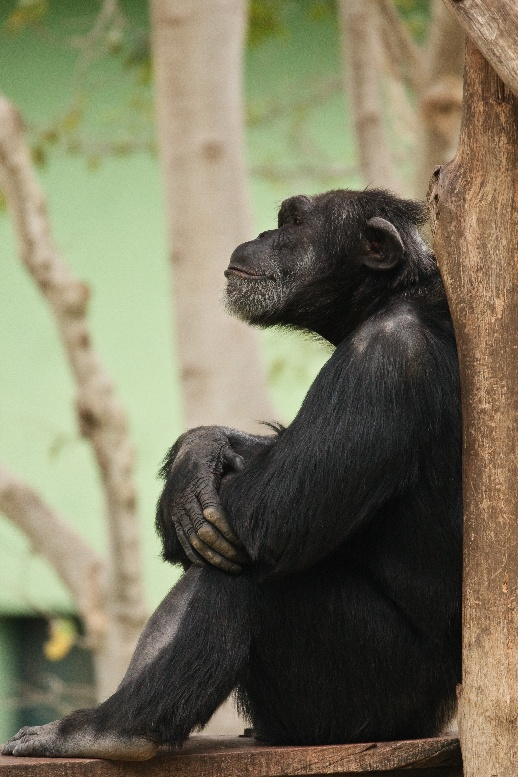
\includegraphics[scale=0.2]{images/monke_512.jpg}
    \\ \small Obraz 4. Oryginalny obraz.

    \vspace{2cm}
    \begin{minipage}{7cm}
        \begin{center}
            \vspace{1cm}
            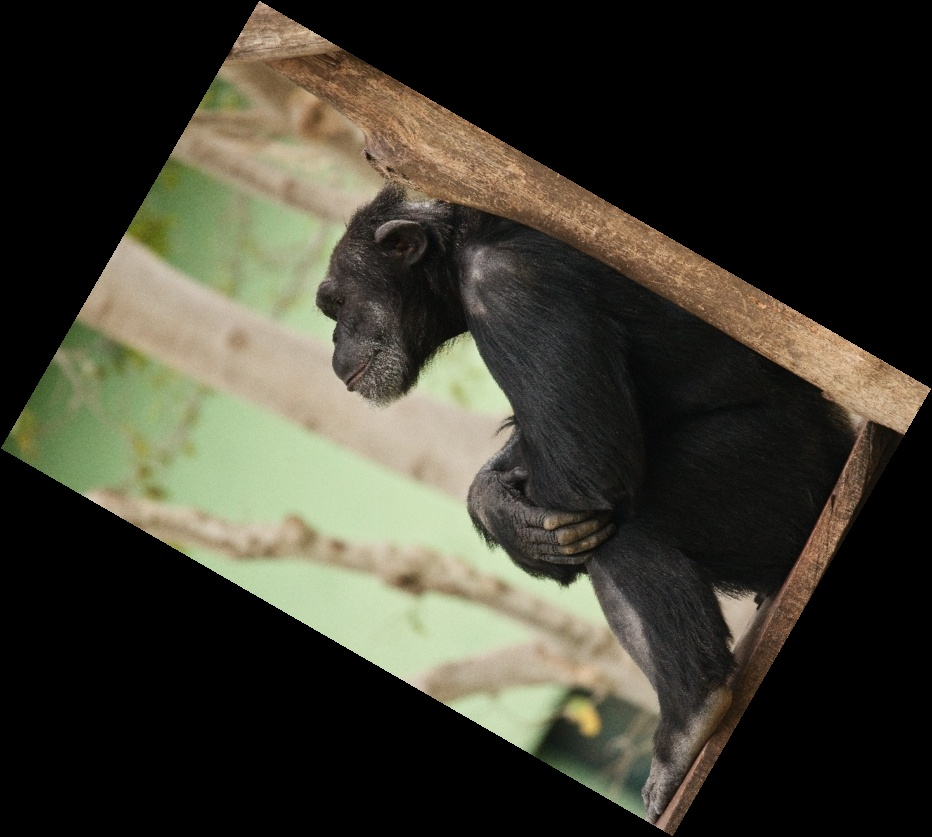
\includegraphics[scale=0.15]{images/rotate_bl_60.jpg}
            \\ \small Obraz 5. Rotacja o 60 stopni za pomocą interpolacji liniowej.
        \end{center}
    \end{minipage}
    \hfill
    \begin{minipage}{7cm}
        \begin{center}
            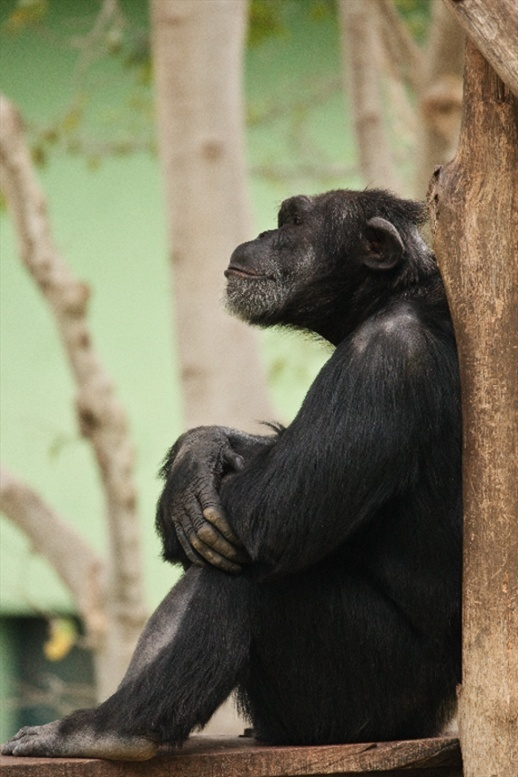
\includegraphics[scale=0.2]{images/5x_BACK_TO_ORG_bc.jpg}
            \\ \small Obraz 6. Rotacja o 360 stopni za pomocą interpolacji liniowej.
      \end{center}
    \end{minipage}
\end{center}


\newpage
\section{Wnioski}
Obiektywnie patrząc, najlepszym algorytmem interpolacji jest sześcienny pod względem płynności 
przejścia między pixelami, a także pozostawia mniej ostre krawędzie, a także nie widać, aż tak urywków
podczas obracania, ale z kolei jest nagorszym pod względem czasu. Najszybszy jest algorytm najbliższego sąsiada,
ale obrazy przekształcane z jego pomocą mogą się wydawać bardziej ostre i posiadać więcej brakujących fragmentów.
Algorytm liniowy jest tylko niewiele wolniejszy od algorytmu najbliższego sąsiada, ale jakością wyjściową
obrazu jest mu znacznie bliżej do algorytmu sześciennego. 

\begin{center}
    \vspace{0.25cm}
    \begin{tabular}{|c|c|c|c|}
        \hline
        & Najbliższy sąsiad & Liniowa & Sześcienna  \\ \hline
        Powiększenie & 0,38s & 4,86s & 55,35s \\ \hline
        Pomniejszenie & 0,27s & 2,77s & 40,51s \\ \hline
        Średni błąd kwadratowy & 55,41 & 33,10 & 23,37 \\ \hline

    \end{tabular}
    \vspace{0.2cm}
    \\ \small Tabela 1. Przedstawiające charakterystyki 
    czasowe oraz błędy typów interpolacji dla skalowania.
\end{center}

\end{document}